% DATA ACQUISITION%

%\Section{Data Acquisition}\label{sec:dataAcqui}

As stated in the introduction \ref{sec:intro}, models are build to estimate the force at the needle tip 
using the OCT data as input.

\subsection{Data}
To gather ground thruth data for modelling and supervised learning, a force sensor is 
integrated into the OCT system by placing it at the end of the needle.

*PICTURE*

Data is collected by poking the needle against a metal plate back and forth in linear or stepwise motions.
The OCT sensor detects the deformation of the transparent material at the tip of the needle that leads to a faster reflection of the light and thus
changes the depth of the maximal reflection in the B-scan.
By this, only frontal forces without any ditributing factors are measured.
The transparent material of the OCT needle deforms up to 0.35mm and one A-scan is represented by 512 pixels.
The acting forces are up to ...(???) Newton by only considering the force in needle direction. (z direction)

\begin{figure}
    \centering
    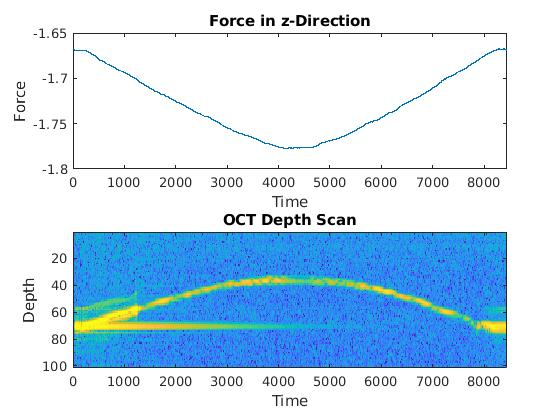
\includegraphics[width=0.8\textwidth]{force_and_oct}
    \caption{asdf}
    \label{fig:force_and_oct}
\end{figure}

\subsection{Preprocessing}

In oder to make use of both data sources, force sensor data is interpolated to obtain the same sampling frequency and start
and end points are synchronized.
The size of the OCT image is reduced to 50 pixels above and below the mean position of the maximum intensities due to
computational reasons. Consequently, the reflection of the repetitive light is neglected.

\subsection{Feature Extraction}

By comparison of the preprocessed OCT depth scans and the low-pass filtered force data it is evident that there is a relationship between the depth at the maximum intensity and the force at each point in time.
Thus, the depth at which the OCT intenity is at its maximum was used as a predictor in the models.
In \cref{fig:force_and_oct} one can observe distortions and artifact in the measured depth scans which threaten to impair the feature extraction if one solely consideres the single depth of the maximum intensity.

These effects were circumvented by considerung multiple depth indices in process of feature extraction.
For each point in time only pixels with an intensity larger than a threshold value were considered.
Pixels at a lower depth were given a preference.
Hence, the constant stripe visible in \cref{fig:force_and_oct} was avoided.
Additionally, an outlier replacement based on the moving mean of the previous depth was performed.
An exemplary feature extraction is depicted in \cref{fig:features_metal}.

\begin{figure}
    \centering
    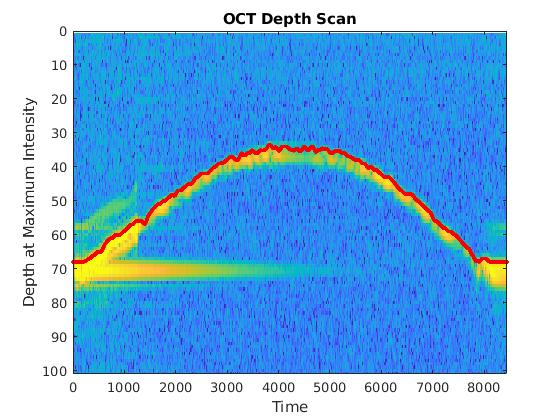
\includegraphics[width=0.8\textwidth]{features_metal}
    \caption{asdf}
    \label{fig:features_metal}
\end{figure}
